% Supplementary material (full results) - FAI Group 22. The 6-page main report is report.tex.
% Results (tables + figures) are generated by:
%   python run_evaluation.py sweep  --preset <tier1|paper> --out results/<sweep>
%   python run_evaluation.py report --sweep-dir results/<sweep> --report-dir Doc/report
% and pulled in via generated/manifest.tex. Compile from this directory.
\documentclass[11pt]{article}

\usepackage[margin=1in]{geometry}
\usepackage[utf8]{inputenc}
\usepackage[T1]{fontenc}
\usepackage{hyperref}
\usepackage{booktabs}
\usepackage{amsmath,amssymb,amsthm,amsfonts}
\usepackage{microtype}
\usepackage{graphicx}
\usepackage[numbers,sort&compress]{natbib}
\usepackage{enumitem}
\usepackage{dsfont}
\usepackage{xcolor}

\theoremstyle{remark}
\newtheorem{remark}{Remark}

\newcommand{\E}{\mathbb{E}}
\newcommand{\ind}[1]{\mathds{1}\!\left[#1\right]}
\newcommand{\Reg}{\mathrm{Reg}}
\newcommand{\BR}{\mathrm{BR}}
\newcommand{\todo}[1]{\textcolor{red}{\textbf{[TODO: #1]}}}

\title{Learning to Bid Under a Budget: A Batched First-Price Ad Auction\\with Unknown Click Probabilities\\[0.4em]\large Supplementary Material: Full Results}
\author{Vivek Raj \and Anvit Aggarwal \and Eshaan Ashish Jaiswal \and Gella Naga Sai Krishna\\[0.3em]
\small IIT Gandhinagar}
\date{}

\begin{document}
\maketitle

\begin{abstract}
We study a repeated batched first-price ad auction in which budget-constrained advertisers submit a full
bid vector over a fixed set of users each round, and must learn their unknown click probabilities from
semi-bandit feedback. With known click probabilities an advertiser's best response is a $0$--$1$ knapsack;
we use it to compute reference equilibria (Tier~1), evaluate budget-aware combinatorial bandit learners
against fixed equilibrium opponents (Tier~2), and simulate all advertisers learning concurrently (Tier~3).
All tiers are evaluated by a shared harness that reports regret, equilibrium gap, distance to equilibrium,
allocation efficiency, profit and revenue with $95\%$ confidence intervals over $30$ seeds, across
$(m,n,\kappa)$ and three round structures.
Thompson sampling is the strongest learner: it has the lowest Tier-2 regret in every canonical cell
(regret slope $\approx0.33$ at $T=1000$, against $0.73$ for UCB with $\alpha=2$), and when all advertisers
use it the final equilibrium gap ($1.46$) is slightly below that of full-information best response.
\end{abstract}

% =====================================================================
\section{Introduction}
Online ad platforms sell many impressions at once to budget-constrained advertisers who do not know in
advance how likely each user is to click. We model this as a batched first-price auction in which each
round is a knapsack problem under uncertainty, connecting auction equilibria with bandits with
knapsacks~\cite{badanidiyuru2013bandits}. The proposal (\texttt{Doc/main.tex}) gives the full
formalization; this report summarizes the model (Section~\ref{sec:model}), documents the evaluation
methodology shared by all tiers (Section~\ref{sec:method}), and reports results
(Section~\ref{sec:results}).

% =====================================================================
\section{Model}\label{sec:model}
Advertisers $a_1,\dots,a_m$ compete over $T$ rounds for users $u_1,\dots,u_n$. In round $t$, $a_i$
submits integer bids $b^t_{ij}\in\{0,\dots,B_i\}$ with $\sum_j b^t_{ij}\le B_i$. The highest positive
bid on $u_j$ wins (ties uniformly at random) and pays its bid; a click
$X_{ij}^t\sim\mathrm{Ber}(f_{ij})$ is worth $v$. Expected profit is
$p_i(b)=\sum_j q_{ij}(b)(f_{ij}v-b_{ij})$, with $q_{ij}$ the winning probability. Learners observe clicks
only on won users, and the highest competing bid $c^t_{-i,j}=\max_{k\ne i}b^t_{kj}$ on every user.

\begin{remark}[Click value]\label{rem:v}
With integer bids and $f_{ij}\le 1$, the cheapest strict win costs $c_{-i,j}+1\ge 1$, so under the
normalisation $v=1$ every item value $r_{ij}=f_{ij}v-c_{-i,j}-1\le 0$ and the unique equilibrium is
``nobody bids''. All experiments therefore use $v=5$ (as in \texttt{run\_tier1.py}), so that a strict win at
price $1$ is profitable whenever $f_{ij}>0.2$.
\end{remark}

% =====================================================================
\section{Evaluation methodology}\label{sec:method}
All tiers run through one harness (\texttt{src/eval}); any agent implementing the shared
\texttt{BaseAdvertiserAgent} interface and registered with \texttt{register\_agent} can be evaluated
unchanged.

\paragraph{Scenarios.} \emph{Tier~1}: every advertiser plays its reference bids $b^*_i$.
\emph{Tier~2}: advertiser $a_1$ runs a learner, all others play $b^*_{-1}$; instances where the Tier-1
solver finds no pure equilibrium are excluded, as in the proposal. \emph{Tier~3}: every advertiser
runs the learner. As a full-information Tier-3 control we also run \texttt{oracle\_br}: each advertiser
knows $f$ and plays the knapsack best response to last round's competing bids, i.e.\ simultaneous
best-response dynamics, which isolates the effect of concurrent adaptation from the effect of learning.

\paragraph{Metrics.} All metrics use the true $f$, never available to agents.
For the profile $b^t$:
\begin{align*}
\text{regret} \quad & \Reg^{(i)}_T=\textstyle\sum_{t} w_t\big(p_i^*(c^t_{-i})-p_i(b^t)\big), \qquad
  p_i^*(c_{-i})=\text{knapsack best-response value},\\
\text{equilibrium gap} \quad & \varepsilon_t=\max_i \max\{0,\ p_i^*(c^t_{-i})-p_i(b^t)\},\\
\text{distance} \quad & \|b^t-b^*\|_1,\qquad
\text{efficiency}\quad \mathrm{Eff}_t=\tfrac1n\textstyle\sum_j\sum_{i\in\arg\max_k f_{kj}} q_{ij}(b^t),\\
\text{revenue / welfare} \quad & \mathrm{Rev}(b^t)=\textstyle\sum_{ij}q_{ij}b^t_{ij},\quad
\mathrm{Wel}(b^t)=\textstyle\sum_{ij}q_{ij}f_{ij}v .
\end{align*}
We also log realized efficiency (with realized wins in place of $q$) and realized profit. ``Final''
values average the last $10\%$ of rounds. The \emph{price of learning} is the Tier-1 value minus the
final learned value. The growth rate of regret is summarised by the least-squares slope of
$\log\Reg_t$ against $\log t$ for $t\ge T/10$: a slope below $1$ indicates sublinear regret ($\approx0.5$
for $\sqrt{T}$-type and $\approx 0$ for logarithmic regret).

\paragraph{Round structures.} \emph{Canonical}: $w_t=1$ and the budget resets each round.
\emph{Discounted}: $w_t=\gamma^{t-1}$ with $\gamma=0.999$; per-round quantities are unchanged and only
cumulative sums are re-weighted. \emph{Cumulative}: advertiser $i$ has a total budget
$\rho\,T B_i$ ($\rho=0.5$), at most $B_i$ per round, and is excluded once it is spent; regret is
measured against the fluid LP benchmark of bandits with knapsacks, which here is $T$ times the
fractional knapsack value at per-round capacity $\min(B_i,\rho B_i)$.

\paragraph{Statistics and instances.} Each configuration is repeated over $30$ seeds; each seed draws a
fresh instance $f_{ij}\sim\mathrm{Beta}(2,5)$ with $B_i=\max(1,\mathrm{round}(\kappa n))$, solves Tier~1
on it, and runs the scenario with independent auction and agent RNG streams. We report means with
Student-$t$ $95\%$ half-widths. Infeasible bid vectors are replaced by zero bids and counted. The grid
is $m\in\{2,3,5\}$, $n\in\{5,10,20,50\}$, $\kappa\in\{0.1,0.25,0.5,1\}$.

\begin{remark}[Nominal vs.\ realised budget tightness]\label{rem:kappa}
The proposal defines $\kappa_i=B_i/\sum_j(c_{-i,j}+1)$, which depends on the equilibrium. The instance
generator instead sets $B_i$ from a nominal $\kappa$ (price $1$ per user). We report both: the realised
$\kappa_i(b^*)$ in the Tier-1 tables is between $0.07$ and $0.65$, so the grid covers scarce to moderate
budgets but never truly abundant ones. Also, for $n=5$ the nominal levels $0.1$ and $0.25$ both
round to $B_i=1$ and give identical instances.
\end{remark}

% =====================================================================
\section{Results}\label{sec:results}
\IfFileExists{generated/manifest.tex}{% Auto-generated from sweep\_tier1 by run_evaluation.py report. Do not edit by hand.

\subsection{Tier 1 across the experimental grid}
Each cell averages 30 random instances (Beta click probabilities, $v=5$); $\pm$ is the 95\% Student-$t$ half-width. Welfare ratio is $\mathrm{Wel}(b^*)$ over the first-best welfare of the omniscient planner.
\begin{figure}[htbp]
\centering
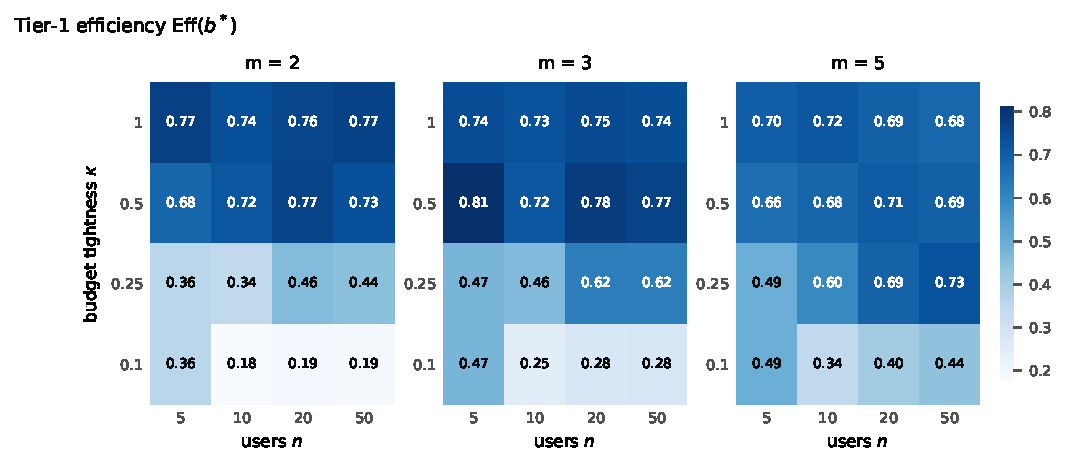
\includegraphics[width=\linewidth]{figures/tier1_t1_efficiency.pdf}
\caption{Tier-1 efficiency $\mathrm{Eff}(b^*)$ across $(m,n,\kappa)$; mean over 30 seeds.}
\label{fig:tier1-t1_efficiency}
\end{figure}

\begin{figure}[htbp]
\centering
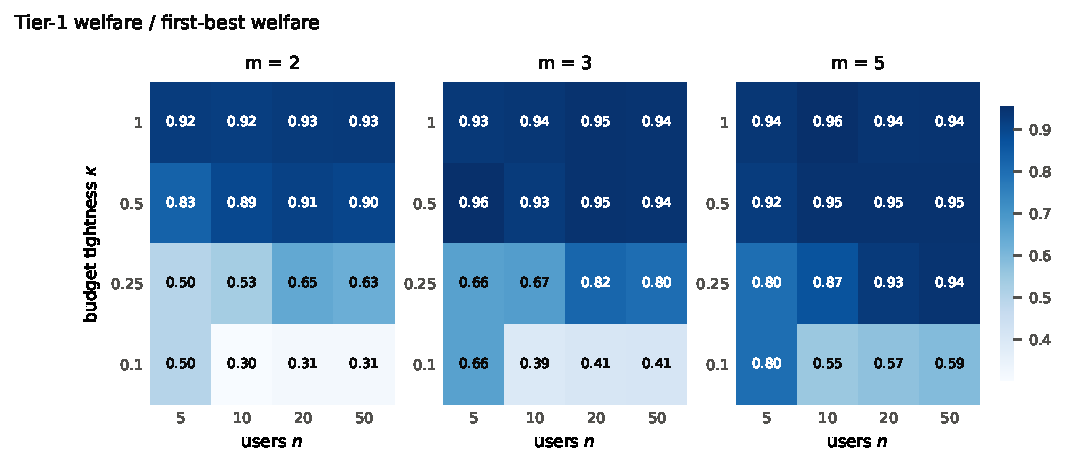
\includegraphics[width=\linewidth]{figures/tier1_t1_welfare_ratio.pdf}
\caption{Tier-1 welfare / first-best welfare across $(m,n,\kappa)$; mean over 30 seeds.}
\label{fig:tier1-t1_welfare_ratio}
\end{figure}

\begin{figure}[htbp]
\centering
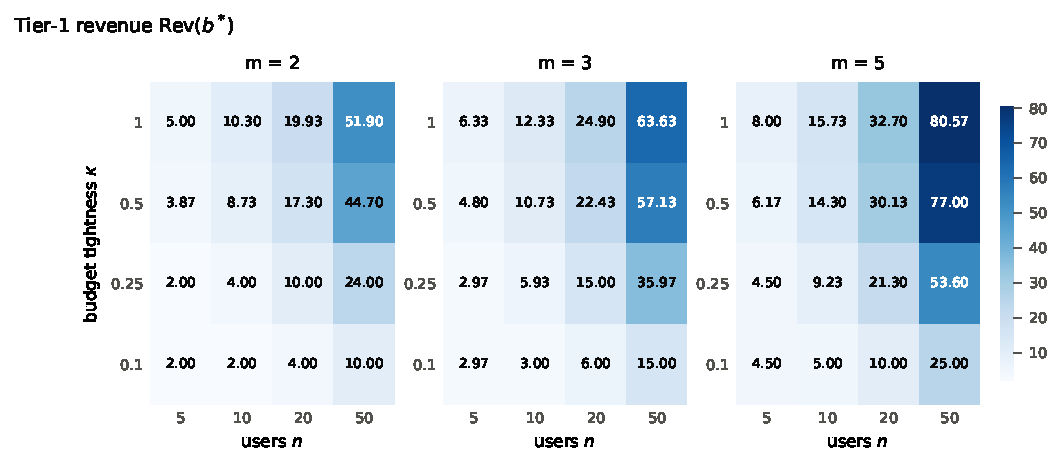
\includegraphics[width=\linewidth]{figures/tier1_t1_revenue.pdf}
\caption{Tier-1 revenue $\mathrm{Rev}(b^*)$ across $(m,n,\kappa)$; mean over 30 seeds.}
\label{fig:tier1-t1_revenue}
\end{figure}

\begin{figure}[htbp]
\centering
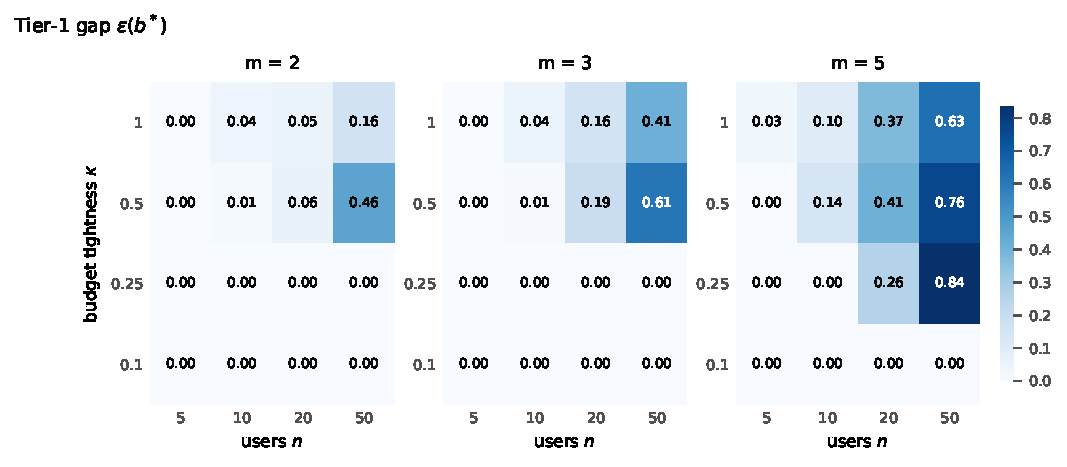
\includegraphics[width=\linewidth]{figures/tier1_t1_eq_gap.pdf}
\caption{Tier-1 gap $\varepsilon(b^*)$ across $(m,n,\kappa)$; mean over 30 seeds.}
\label{fig:tier1-t1_eq_gap}
\end{figure}

\begin{table}[htbp]
\centering
\scriptsize
\caption{Tier-1 reference profile, $m=2$ advertisers.}
\label{tab:tier1_m2}
\begin{tabular}{@{}rrrccccccc@{}}
\toprule
m & n & $\kappa$ & $B_i$ & $\kappa_i(b^*)$ & pure & $\varepsilon(b^*)$ & Rev & Eff & Wel/FB \\
\midrule
2 & 5 & 0.1 & $1 \pm 0$ & $0.17 \pm 0.00$ & $1.00 \pm 0.00$ & $0.00 \pm 0.00$ & $2.00 \pm 0.00$ & $0.36 \pm 0.03$ & $0.50 \pm 0.02$ \\
2 & 5 & 0.25 & $1 \pm 0$ & $0.17 \pm 0.00$ & $1.00 \pm 0.00$ & $0.00 \pm 0.00$ & $2.00 \pm 0.00$ & $0.36 \pm 0.03$ & $0.50 \pm 0.02$ \\
2 & 5 & 0.5 & $2 \pm 0$ & $0.29 \pm 0.00$ & $1.00 \pm 0.00$ & $0.00 \pm 0.00$ & $3.87 \pm 0.13$ & $0.68 \pm 0.05$ & $0.83 \pm 0.02$ \\
2 & 5 & 1 & $5 \pm 0$ & $0.65 \pm 0.03$ & $1.00 \pm 0.00$ & $0.00 \pm 0.00$ & $5.00 \pm 0.35$ & $0.77 \pm 0.08$ & $0.92 \pm 0.04$ \\
2 & 10 & 0.1 & $1 \pm 0$ & $0.09 \pm 0.00$ & $1.00 \pm 0.00$ & $0.00 \pm 0.00$ & $2.00 \pm 0.00$ & $0.18 \pm 0.02$ & $0.30 \pm 0.02$ \\
2 & 10 & 0.25 & $2 \pm 0$ & $0.17 \pm 0.00$ & $1.00 \pm 0.00$ & $0.00 \pm 0.00$ & $4.00 \pm 0.00$ & $0.34 \pm 0.03$ & $0.53 \pm 0.02$ \\
2 & 10 & 0.5 & $5 \pm 0$ & $0.34 \pm 0.00$ & $0.90 \pm 0.00$ & $0.01 \pm 0.02$ & $8.73 \pm 0.32$ & $0.72 \pm 0.07$ & $0.89 \pm 0.03$ \\
2 & 10 & 1 & $10 \pm 0$ & $0.63 \pm 0.02$ & $0.90 \pm 0.00$ & $0.04 \pm 0.05$ & $10.30 \pm 0.59$ & $0.74 \pm 0.07$ & $0.92 \pm 0.02$ \\
2 & 20 & 0.1 & $2 \pm 0$ & $0.09 \pm 0.00$ & $1.00 \pm 0.00$ & $0.00 \pm 0.00$ & $4.00 \pm 0.00$ & $0.19 \pm 0.01$ & $0.31 \pm 0.01$ \\
2 & 20 & 0.25 & $5 \pm 0$ & $0.20 \pm 0.00$ & $1.00 \pm 0.00$ & $0.00 \pm 0.00$ & $10.00 \pm 0.00$ & $0.46 \pm 0.01$ & $0.65 \pm 0.01$ \\
2 & 20 & 0.5 & $10 \pm 0$ & $0.35 \pm 0.00$ & $0.77 \pm 0.00$ & $0.06 \pm 0.05$ & $17.30 \pm 0.54$ & $0.77 \pm 0.03$ & $0.91 \pm 0.01$ \\
2 & 20 & 1 & $20 \pm 0$ & $0.65 \pm 0.02$ & $0.90 \pm 0.00$ & $0.05 \pm 0.08$ & $19.93 \pm 0.89$ & $0.76 \pm 0.03$ & $0.93 \pm 0.01$ \\
2 & 50 & 0.1 & $5 \pm 0$ & $0.09 \pm 0.00$ & $1.00 \pm 0.00$ & $0.00 \pm 0.00$ & $10.00 \pm 0.00$ & $0.19 \pm 0.01$ & $0.31 \pm 0.01$ \\
2 & 50 & 0.25 & $12 \pm 0$ & $0.19 \pm 0.00$ & $1.00 \pm 0.00$ & $0.00 \pm 0.00$ & $24.00 \pm 0.00$ & $0.44 \pm 0.01$ & $0.63 \pm 0.01$ \\
2 & 50 & 0.5 & $25 \pm 0$ & $0.34 \pm 0.00$ & $0.30 \pm 0.00$ & $0.46 \pm 0.18$ & $44.70 \pm 0.71$ & $0.73 \pm 0.03$ & $0.90 \pm 0.01$ \\
2 & 50 & 1 & $50 \pm 0$ & $0.63 \pm 0.01$ & $0.57 \pm 0.00$ & $0.16 \pm 0.09$ & $51.90 \pm 1.53$ & $0.77 \pm 0.03$ & $0.93 \pm 0.01$ \\
\bottomrule
\end{tabular}
\end{table}

\begin{table}[htbp]
\centering
\scriptsize
\caption{Tier-1 reference profile, $m=3$ advertisers.}
\label{tab:tier1_m3}
\begin{tabular}{@{}rrrccccccc@{}}
\toprule
m & n & $\kappa$ & $B_i$ & $\kappa_i(b^*)$ & pure & $\varepsilon(b^*)$ & Rev & Eff & Wel/FB \\
\midrule
3 & 5 & 0.1 & $1 \pm 0$ & $0.14 \pm 0.00$ & $1.00 \pm 0.00$ & $0.00 \pm 0.00$ & $2.97 \pm 0.07$ & $0.47 \pm 0.05$ & $0.66 \pm 0.02$ \\
3 & 5 & 0.25 & $1 \pm 0$ & $0.14 \pm 0.00$ & $1.00 \pm 0.00$ & $0.00 \pm 0.00$ & $2.97 \pm 0.07$ & $0.47 \pm 0.05$ & $0.66 \pm 0.02$ \\
3 & 5 & 0.5 & $2 \pm 0$ & $0.24 \pm 0.00$ & $1.00 \pm 0.00$ & $0.00 \pm 0.00$ & $4.80 \pm 0.15$ & $0.81 \pm 0.06$ & $0.96 \pm 0.02$ \\
3 & 5 & 1 & $5 \pm 0$ & $0.52 \pm 0.02$ & $1.00 \pm 0.00$ & $0.00 \pm 0.00$ & $6.33 \pm 0.38$ & $0.74 \pm 0.07$ & $0.93 \pm 0.02$ \\
3 & 10 & 0.1 & $1 \pm 0$ & $0.08 \pm 0.00$ & $1.00 \pm 0.00$ & $0.00 \pm 0.00$ & $3.00 \pm 0.00$ & $0.25 \pm 0.03$ & $0.39 \pm 0.01$ \\
3 & 10 & 0.25 & $2 \pm 0$ & $0.14 \pm 0.00$ & $1.00 \pm 0.00$ & $0.00 \pm 0.00$ & $5.93 \pm 0.14$ & $0.46 \pm 0.05$ & $0.67 \pm 0.02$ \\
3 & 10 & 0.5 & $5 \pm 0$ & $0.29 \pm 0.01$ & $0.90 \pm 0.00$ & $0.01 \pm 0.01$ & $10.73 \pm 0.45$ & $0.72 \pm 0.05$ & $0.93 \pm 0.02$ \\
3 & 10 & 1 & $10 \pm 0$ & $0.53 \pm 0.02$ & $0.87 \pm 0.00$ & $0.04 \pm 0.05$ & $12.33 \pm 0.58$ & $0.73 \pm 0.06$ & $0.94 \pm 0.02$ \\
3 & 20 & 0.1 & $2 \pm 0$ & $0.08 \pm 0.00$ & $1.00 \pm 0.00$ & $0.00 \pm 0.00$ & $6.00 \pm 0.00$ & $0.28 \pm 0.01$ & $0.41 \pm 0.01$ \\
3 & 20 & 0.25 & $5 \pm 0$ & $0.17 \pm 0.00$ & $1.00 \pm 0.00$ & $0.00 \pm 0.00$ & $15.00 \pm 0.00$ & $0.62 \pm 0.02$ & $0.82 \pm 0.01$ \\
3 & 20 & 0.5 & $10 \pm 0$ & $0.28 \pm 0.00$ & $0.47 \pm 0.00$ & $0.19 \pm 0.10$ & $22.43 \pm 0.61$ & $0.78 \pm 0.04$ & $0.95 \pm 0.01$ \\
3 & 20 & 1 & $20 \pm 0$ & $0.52 \pm 0.01$ & $0.73 \pm 0.00$ & $0.16 \pm 0.13$ & $24.90 \pm 0.85$ & $0.75 \pm 0.04$ & $0.95 \pm 0.01$ \\
3 & 50 & 0.1 & $5 \pm 0$ & $0.08 \pm 0.00$ & $1.00 \pm 0.00$ & $0.00 \pm 0.00$ & $15.00 \pm 0.00$ & $0.28 \pm 0.01$ & $0.41 \pm 0.00$ \\
3 & 50 & 0.25 & $12 \pm 0$ & $0.16 \pm 0.00$ & $1.00 \pm 0.00$ & $0.00 \pm 0.00$ & $35.97 \pm 0.07$ & $0.62 \pm 0.02$ & $0.80 \pm 0.01$ \\
3 & 50 & 0.5 & $25 \pm 0$ & $0.27 \pm 0.00$ & $0.20 \pm 0.00$ & $0.61 \pm 0.22$ & $57.13 \pm 1.34$ & $0.77 \pm 0.02$ & $0.94 \pm 0.01$ \\
3 & 50 & 1 & $50 \pm 0$ & $0.51 \pm 0.01$ & $0.37 \pm 0.00$ & $0.41 \pm 0.19$ & $63.63 \pm 1.70$ & $0.74 \pm 0.03$ & $0.94 \pm 0.01$ \\
\bottomrule
\end{tabular}
\end{table}

\begin{table}[htbp]
\centering
\scriptsize
\caption{Tier-1 reference profile, $m=5$ advertisers.}
\label{tab:tier1_m5}
\begin{tabular}{@{}rrrccccccc@{}}
\toprule
m & n & $\kappa$ & $B_i$ & $\kappa_i(b^*)$ & pure & $\varepsilon(b^*)$ & Rev & Eff & Wel/FB \\
\midrule
5 & 5 & 0.1 & $1 \pm 0$ & $0.12 \pm 0.00$ & $1.00 \pm 0.00$ & $0.00 \pm 0.00$ & $4.50 \pm 0.21$ & $0.49 \pm 0.07$ & $0.80 \pm 0.04$ \\
5 & 5 & 0.25 & $1 \pm 0$ & $0.12 \pm 0.00$ & $1.00 \pm 0.00$ & $0.00 \pm 0.00$ & $4.50 \pm 0.21$ & $0.49 \pm 0.07$ & $0.80 \pm 0.04$ \\
5 & 5 & 0.5 & $2 \pm 0$ & $0.20 \pm 0.00$ & $0.97 \pm 0.00$ & $0.00 \pm 0.00$ & $6.17 \pm 0.22$ & $0.66 \pm 0.07$ & $0.92 \pm 0.02$ \\
5 & 5 & 1 & $5 \pm 0$ & $0.42 \pm 0.02$ & $0.87 \pm 0.00$ & $0.03 \pm 0.04$ & $8.00 \pm 0.50$ & $0.70 \pm 0.06$ & $0.94 \pm 0.02$ \\
5 & 10 & 0.1 & $1 \pm 0$ & $0.07 \pm 0.00$ & $1.00 \pm 0.00$ & $0.00 \pm 0.00$ & $5.00 \pm 0.00$ & $0.34 \pm 0.05$ & $0.55 \pm 0.01$ \\
5 & 10 & 0.25 & $2 \pm 0$ & $0.11 \pm 0.00$ & $1.00 \pm 0.00$ & $0.00 \pm 0.00$ & $9.23 \pm 0.21$ & $0.60 \pm 0.05$ & $0.87 \pm 0.02$ \\
5 & 10 & 0.5 & $5 \pm 0$ & $0.23 \pm 0.01$ & $0.73 \pm 0.00$ & $0.14 \pm 0.11$ & $14.30 \pm 0.59$ & $0.68 \pm 0.06$ & $0.95 \pm 0.01$ \\
5 & 10 & 1 & $10 \pm 0$ & $0.42 \pm 0.01$ & $0.73 \pm 0.00$ & $0.10 \pm 0.11$ & $15.73 \pm 0.59$ & $0.72 \pm 0.06$ & $0.96 \pm 0.01$ \\
5 & 20 & 0.1 & $2 \pm 0$ & $0.07 \pm 0.00$ & $1.00 \pm 0.00$ & $0.00 \pm 0.00$ & $10.00 \pm 0.00$ & $0.40 \pm 0.02$ & $0.57 \pm 0.01$ \\
5 & 20 & 0.25 & $5 \pm 0$ & $0.13 \pm 0.00$ & $0.30 \pm 0.00$ & $0.26 \pm 0.09$ & $21.30 \pm 0.24$ & $0.69 \pm 0.04$ & $0.93 \pm 0.01$ \\
5 & 20 & 0.5 & $10 \pm 0$ & $0.22 \pm 0.00$ & $0.23 \pm 0.00$ & $0.41 \pm 0.16$ & $30.13 \pm 0.81$ & $0.71 \pm 0.04$ & $0.95 \pm 0.01$ \\
5 & 20 & 1 & $20 \pm 0$ & $0.41 \pm 0.01$ & $0.33 \pm 0.00$ & $0.37 \pm 0.19$ & $32.70 \pm 0.97$ & $0.69 \pm 0.04$ & $0.94 \pm 0.01$ \\
5 & 50 & 0.1 & $5 \pm 0$ & $0.07 \pm 0.00$ & $1.00 \pm 0.00$ & $0.00 \pm 0.00$ & $25.00 \pm 0.00$ & $0.44 \pm 0.01$ & $0.59 \pm 0.00$ \\
5 & 50 & 0.25 & $12 \pm 0$ & $0.13 \pm 0.00$ & $0.00 \pm 0.00$ & $0.84 \pm 0.15$ & $53.60 \pm 0.35$ & $0.73 \pm 0.02$ & $0.94 \pm 0.01$ \\
5 & 50 & 0.5 & $25 \pm 0$ & $0.21 \pm 0.00$ & $0.03 \pm 0.00$ & $0.76 \pm 0.25$ & $77.00 \pm 1.19$ & $0.69 \pm 0.03$ & $0.95 \pm 0.01$ \\
5 & 50 & 1 & $50 \pm 0$ & $0.42 \pm 0.01$ & $0.20 \pm 0.00$ & $0.63 \pm 0.27$ & $80.57 \pm 1.47$ & $0.68 \pm 0.03$ & $0.94 \pm 0.01$ \\
\bottomrule
\end{tabular}
\end{table}

\clearpage
\subsection{Tier 3: all advertisers adapt concurrently}
\begin{figure}[htbp]
\centering
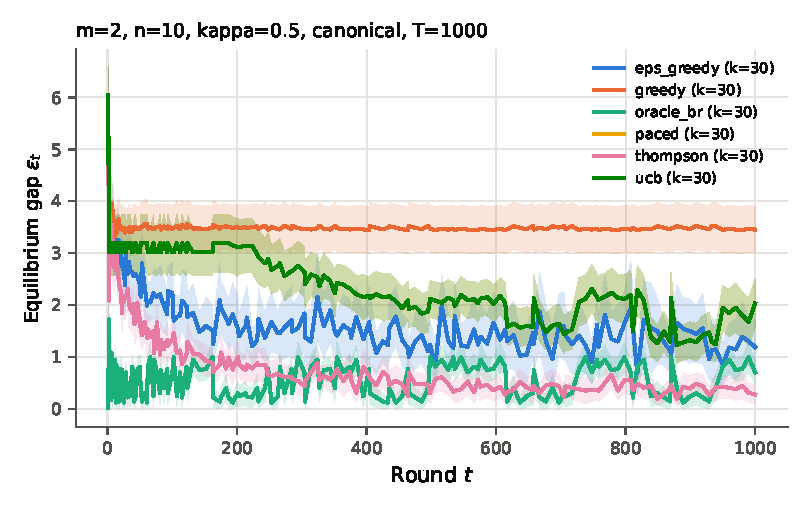
\includegraphics[width=0.8\linewidth]{figures/tier3_curves_eq_gap.pdf}
\caption{Equilibrium gap $\varepsilon_t$ vs.\ round, mean and 95\% CI band over seeds ($m=2$, $n=10$, $\kappa=0.5$, canonical).}
\label{fig:tier3-eq_gap}
\end{figure}

\begin{figure}[htbp]
\centering
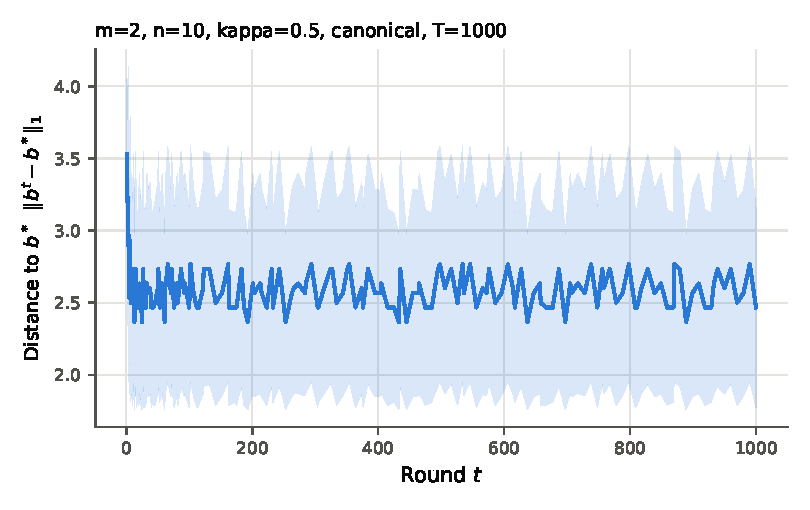
\includegraphics[width=0.8\linewidth]{figures/tier3_curves_eq_distance.pdf}
\caption{Distance to $b^*$  $\|b^t-b^*\|_1$ vs.\ round, mean and 95\% CI band over seeds ($m=2$, $n=10$, $\kappa=0.5$, canonical).}
\label{fig:tier3-eq_distance}
\end{figure}

\begin{figure}[htbp]
\centering
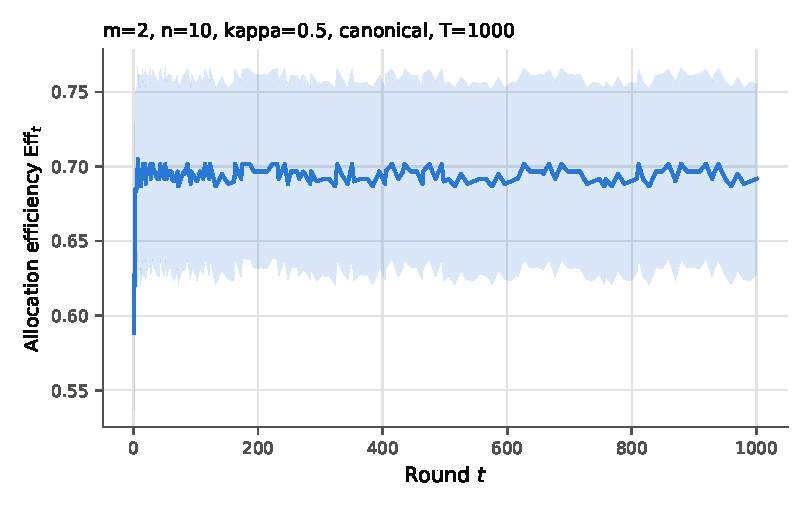
\includegraphics[width=0.8\linewidth]{figures/tier3_curves_efficiency.pdf}
\caption{Allocation efficiency $\mathrm{Eff}_t$ vs.\ round, mean and 95\% CI band over seeds ($m=2$, $n=10$, $\kappa=0.5$, canonical).}
\label{fig:tier3-efficiency}
\end{figure}

\begin{figure}[htbp]
\centering
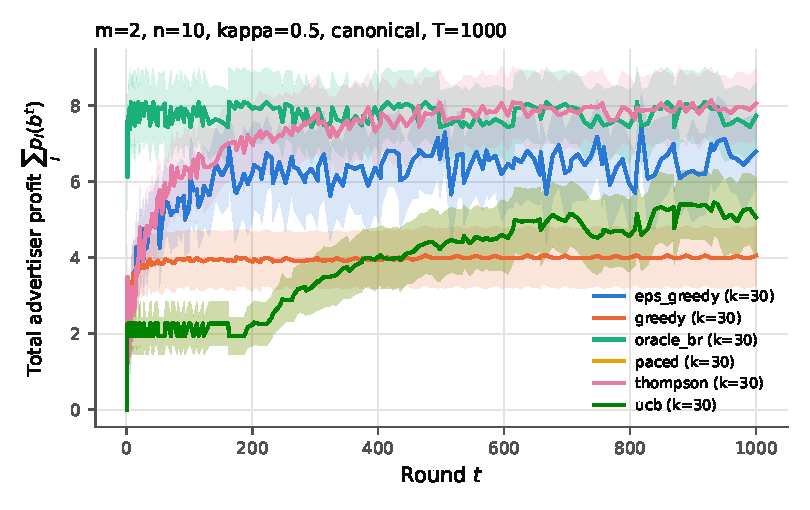
\includegraphics[width=0.8\linewidth]{figures/tier3_curves_total_profit.pdf}
\caption{Total advertiser profit $\sum_i p_i(b^t)$ vs.\ round, mean and 95\% CI band over seeds ($m=2$, $n=10$, $\kappa=0.5$, canonical).}
\label{fig:tier3-total_profit}
\end{figure}

\begin{figure}[htbp]
\centering
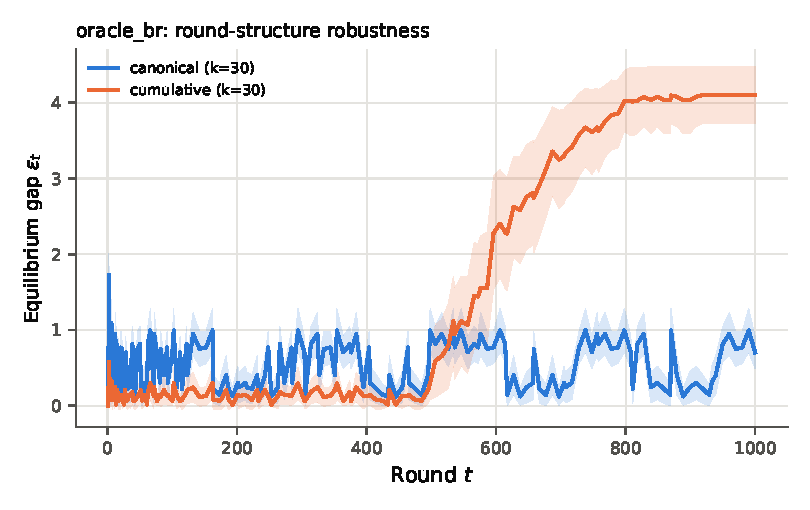
\includegraphics[width=0.8\linewidth]{figures/tier3_oracle_br_structures_eq_gap.pdf}
\caption{\texttt{oracle\_br}: Equilibrium gap $\varepsilon_t$ under different round structures (cumulative is measured against the fluid LP benchmark; the discounted variant changes only cumulative sums, so its per-round curve equals canonical).}
\label{fig:tier3-oracle_br-structures}
\end{figure}

\begin{figure}[htbp]
\centering
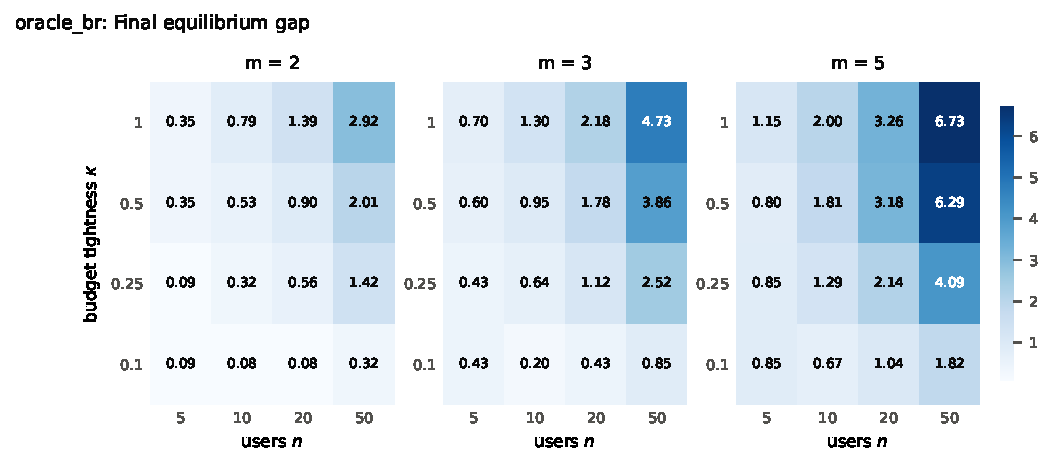
\includegraphics[width=\linewidth]{figures/tier3_oracle_br_heat_eq_gap_last.pdf}
\caption{\texttt{oracle\_br} (tier3, canonical): Final equilibrium gap across $(m,n,\kappa)$.}
\label{fig:tier3-oracle_br-eq_gap_last}
\end{figure}

\begin{figure}[htbp]
\centering
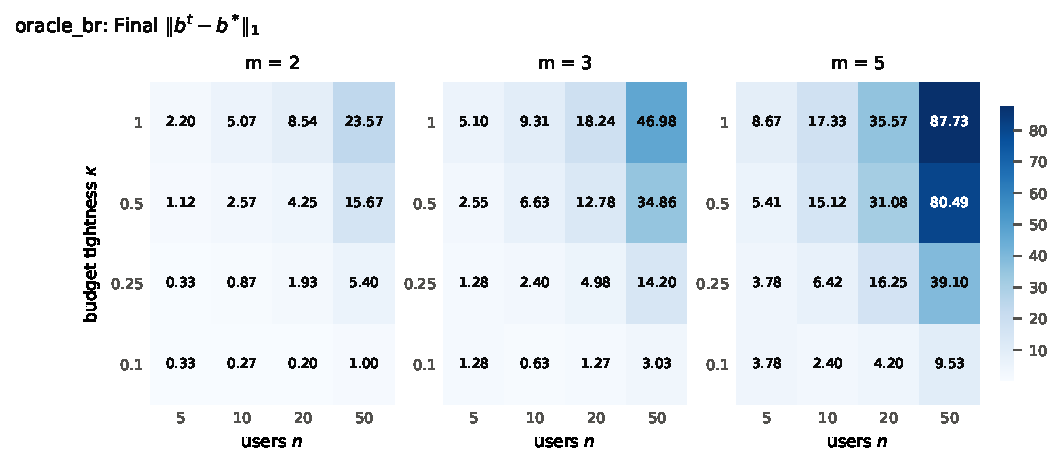
\includegraphics[width=\linewidth]{figures/tier3_oracle_br_heat_eq_distance_last.pdf}
\caption{\texttt{oracle\_br} (tier3, canonical): Final $\|b^t-b^*\|_1$ across $(m,n,\kappa)$.}
\label{fig:tier3-oracle_br-eq_distance_last}
\end{figure}

\begin{figure}[htbp]
\centering
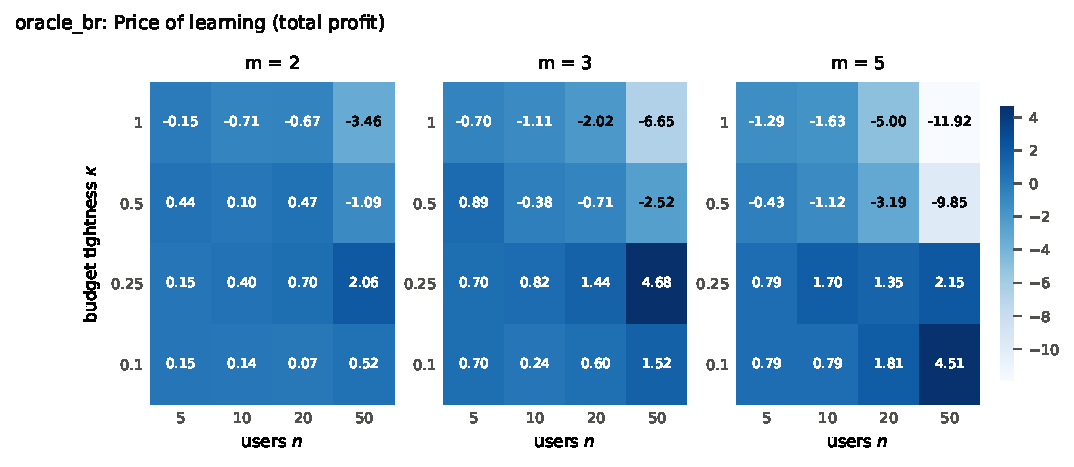
\includegraphics[width=\linewidth]{figures/tier3_oracle_br_heat_pol_total_profit.pdf}
\caption{\texttt{oracle\_br} (tier3, canonical): Price of learning (total profit) across $(m,n,\kappa)$.}
\label{fig:tier3-oracle_br-pol_total_profit}
\end{figure}

\begin{figure}[htbp]
\centering
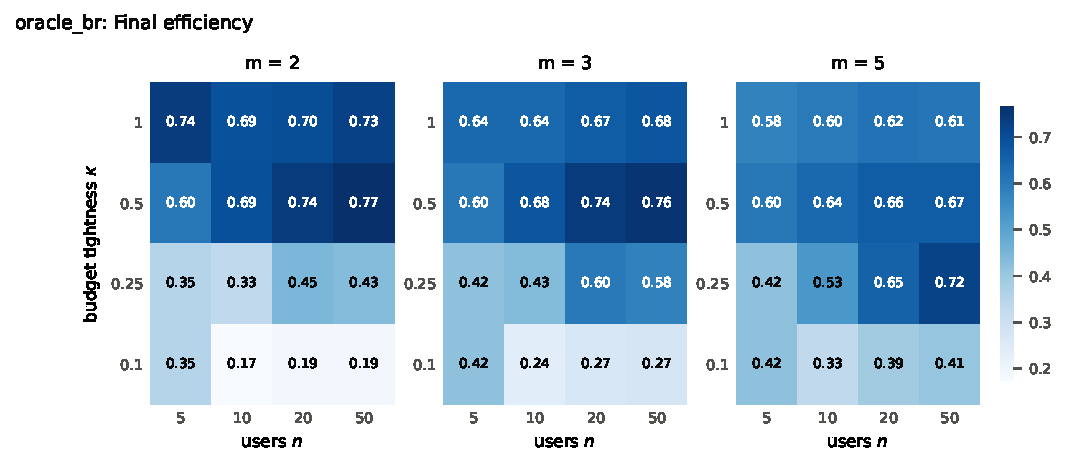
\includegraphics[width=\linewidth]{figures/tier3_oracle_br_heat_efficiency_last.pdf}
\caption{\texttt{oracle\_br} (tier3, canonical): Final efficiency across $(m,n,\kappa)$.}
\label{fig:tier3-oracle_br-efficiency_last}
\end{figure}

\begin{table}[htbp]
\centering
\scriptsize
\caption{\texttt{oracle\_br}, tier3, canonical round structure, $T=1000$ (final metrics averaged over the last 10\% of rounds; PoL = Tier-1 minus learned).}
\label{tab:tier3_oracle_br_canonical}
\begin{tabular}{@{}rrrcccccc@{}}
\toprule
m & n & $\kappa$ & $\varepsilon$ & $\|b-b^*\|_1$ & Eff & Rev & PoL$_\pi$ & PoL$_\mathrm{Eff}$ \\
\midrule
2 & 5 & 0.1 & $0.09 \pm 0.08$ & $0.3 \pm 0.3$ & $0.35 \pm 0.03$ & $1.90 \pm 0.09$ & $0.15 \pm 0.14$ & $0.01 \pm 0.02$ \\
2 & 5 & 0.25 & $0.09 \pm 0.08$ & $0.3 \pm 0.3$ & $0.35 \pm 0.03$ & $1.90 \pm 0.09$ & $0.15 \pm 0.14$ & $0.01 \pm 0.02$ \\
2 & 5 & 0.5 & $0.35 \pm 0.14$ & $1.1 \pm 0.4$ & $0.60 \pm 0.06$ & $3.30 \pm 0.25$ & $0.44 \pm 0.22$ & $0.08 \pm 0.04$ \\
2 & 5 & 1 & $0.35 \pm 0.13$ & $2.2 \pm 0.5$ & $0.74 \pm 0.07$ & $4.22 \pm 0.40$ & $-0.15 \pm 0.22$ & $0.03 \pm 0.04$ \\
2 & 10 & 0.1 & $0.08 \pm 0.08$ & $0.3 \pm 0.3$ & $0.17 \pm 0.02$ & $1.93 \pm 0.06$ & $0.14 \pm 0.14$ & $0.00 \pm 0.01$ \\
2 & 10 & 0.25 & $0.32 \pm 0.16$ & $0.9 \pm 0.4$ & $0.33 \pm 0.03$ & $3.70 \pm 0.16$ & $0.40 \pm 0.23$ & $0.01 \pm 0.02$ \\
2 & 10 & 0.5 & $0.53 \pm 0.13$ & $2.6 \pm 0.7$ & $0.69 \pm 0.06$ & $7.82 \pm 0.42$ & $0.10 \pm 0.33$ & $0.03 \pm 0.03$ \\
2 & 10 & 1 & $0.79 \pm 0.15$ & $5.1 \pm 0.8$ & $0.69 \pm 0.06$ & $7.92 \pm 0.54$ & $-0.71 \pm 0.39$ & $0.05 \pm 0.03$ \\
2 & 20 & 0.1 & $0.08 \pm 0.09$ & $0.2 \pm 0.2$ & $0.19 \pm 0.01$ & $3.95 \pm 0.06$ & $0.07 \pm 0.09$ & $0.00 \pm 0.00$ \\
2 & 20 & 0.25 & $0.56 \pm 0.20$ & $1.9 \pm 0.6$ & $0.45 \pm 0.01$ & $9.43 \pm 0.19$ & $0.70 \pm 0.26$ & $0.01 \pm 0.01$ \\
2 & 20 & 0.5 & $0.90 \pm 0.16$ & $4.3 \pm 0.8$ & $0.74 \pm 0.03$ & $16.14 \pm 0.56$ & $0.47 \pm 0.45$ & $0.02 \pm 0.02$ \\
2 & 20 & 1 & $1.39 \pm 0.17$ & $8.5 \pm 1.1$ & $0.70 \pm 0.03$ & $15.90 \pm 0.69$ & $-0.67 \pm 0.55$ & $0.06 \pm 0.02$ \\
2 & 50 & 0.1 & $0.32 \pm 0.17$ & $1.0 \pm 0.5$ & $0.19 \pm 0.01$ & $9.72 \pm 0.15$ & $0.52 \pm 0.29$ & $0.00 \pm 0.00$ \\
2 & 50 & 0.25 & $1.42 \pm 0.19$ & $5.4 \pm 0.7$ & $0.43 \pm 0.01$ & $22.53 \pm 0.20$ & $2.06 \pm 0.30$ & $0.01 \pm 0.01$ \\
2 & 50 & 0.5 & $2.01 \pm 0.24$ & $15.7 \pm 2.6$ & $0.77 \pm 0.02$ & $42.25 \pm 1.01$ & $-1.09 \pm 0.79$ & $-0.03 \pm 0.02$ \\
2 & 50 & 1 & $2.92 \pm 0.26$ & $23.6 \pm 2.1$ & $0.73 \pm 0.02$ & $41.18 \pm 1.17$ & $-3.46 \pm 0.92$ & $0.04 \pm 0.01$ \\
\midrule
3 & 5 & 0.1 & $0.43 \pm 0.14$ & $1.3 \pm 0.5$ & $0.42 \pm 0.06$ & $2.47 \pm 0.19$ & $0.70 \pm 0.24$ & $0.06 \pm 0.04$ \\
3 & 5 & 0.25 & $0.43 \pm 0.14$ & $1.3 \pm 0.5$ & $0.42 \pm 0.06$ & $2.47 \pm 0.19$ & $0.70 \pm 0.24$ & $0.06 \pm 0.04$ \\
3 & 5 & 0.5 & $0.60 \pm 0.15$ & $2.5 \pm 0.6$ & $0.60 \pm 0.08$ & $3.77 \pm 0.28$ & $0.89 \pm 0.30$ & $0.21 \pm 0.06$ \\
3 & 5 & 1 & $0.70 \pm 0.15$ & $5.1 \pm 0.8$ & $0.64 \pm 0.06$ & $4.24 \pm 0.28$ & $-0.70 \pm 0.40$ & $0.10 \pm 0.04$ \\
3 & 10 & 0.1 & $0.20 \pm 0.14$ & $0.6 \pm 0.4$ & $0.24 \pm 0.03$ & $2.85 \pm 0.10$ & $0.24 \pm 0.17$ & $0.01 \pm 0.01$ \\
3 & 10 & 0.25 & $0.64 \pm 0.17$ & $2.4 \pm 0.7$ & $0.43 \pm 0.04$ & $5.25 \pm 0.22$ & $0.82 \pm 0.28$ & $0.03 \pm 0.03$ \\
3 & 10 & 0.5 & $0.95 \pm 0.16$ & $6.6 \pm 1.0$ & $0.68 \pm 0.05$ & $8.67 \pm 0.43$ & $-0.38 \pm 0.49$ & $0.04 \pm 0.04$ \\
3 & 10 & 1 & $1.30 \pm 0.17$ & $9.3 \pm 0.9$ & $0.64 \pm 0.05$ & $8.31 \pm 0.48$ & $-1.11 \pm 0.41$ & $0.09 \pm 0.04$ \\
3 & 20 & 0.1 & $0.43 \pm 0.16$ & $1.3 \pm 0.5$ & $0.27 \pm 0.01$ & $5.67 \pm 0.12$ & $0.60 \pm 0.24$ & $0.01 \pm 0.01$ \\
3 & 20 & 0.25 & $1.12 \pm 0.14$ & $5.0 \pm 0.8$ & $0.60 \pm 0.02$ & $13.47 \pm 0.27$ & $1.44 \pm 0.36$ & $0.02 \pm 0.02$ \\
3 & 20 & 0.5 & $1.78 \pm 0.18$ & $12.8 \pm 1.5$ & $0.74 \pm 0.03$ & $18.51 \pm 0.67$ & $-0.71 \pm 0.67$ & $0.04 \pm 0.03$ \\
3 & 20 & 1 & $2.18 \pm 0.20$ & $18.2 \pm 1.5$ & $0.67 \pm 0.04$ & $17.31 \pm 0.71$ & $-2.02 \pm 0.62$ & $0.08 \pm 0.03$ \\
3 & 50 & 0.1 & $0.85 \pm 0.21$ & $3.0 \pm 0.7$ & $0.27 \pm 0.01$ & $14.20 \pm 0.19$ & $1.52 \pm 0.41$ & $0.01 \pm 0.01$ \\
3 & 50 & 0.25 & $2.52 \pm 0.27$ & $14.2 \pm 1.2$ & $0.58 \pm 0.02$ & $31.80 \pm 0.46$ & $4.68 \pm 0.82$ & $0.04 \pm 0.02$ \\
3 & 50 & 0.5 & $3.86 \pm 0.29$ & $34.9 \pm 3.3$ & $0.76 \pm 0.02$ & $47.19 \pm 1.24$ & $-2.52 \pm 1.53$ & $0.01 \pm 0.02$ \\
3 & 50 & 1 & $4.73 \pm 0.37$ & $47.0 \pm 3.0$ & $0.68 \pm 0.02$ & $44.23 \pm 1.16$ & $-6.65 \pm 1.12$ & $0.06 \pm 0.02$ \\
\midrule
5 & 5 & 0.1 & $0.85 \pm 0.13$ & $3.8 \pm 0.7$ & $0.42 \pm 0.06$ & $3.45 \pm 0.30$ & $0.79 \pm 0.53$ & $0.07 \pm 0.08$ \\
5 & 5 & 0.25 & $0.85 \pm 0.13$ & $3.8 \pm 0.7$ & $0.42 \pm 0.06$ & $3.45 \pm 0.30$ & $0.79 \pm 0.53$ & $0.07 \pm 0.08$ \\
5 & 5 & 0.5 & $0.80 \pm 0.19$ & $5.4 \pm 1.0$ & $0.60 \pm 0.06$ & $4.31 \pm 0.18$ & $-0.43 \pm 0.34$ & $0.06 \pm 0.07$ \\
5 & 5 & 1 & $1.15 \pm 0.18$ & $8.7 \pm 0.8$ & $0.58 \pm 0.06$ & $4.76 \pm 0.30$ & $-1.29 \pm 0.41$ & $0.12 \pm 0.06$ \\
5 & 10 & 0.1 & $0.67 \pm 0.18$ & $2.4 \pm 0.7$ & $0.33 \pm 0.04$ & $4.37 \pm 0.21$ & $0.79 \pm 0.26$ & $0.01 \pm 0.02$ \\
5 & 10 & 0.25 & $1.29 \pm 0.17$ & $6.4 \pm 0.9$ & $0.53 \pm 0.05$ & $7.13 \pm 0.35$ & $1.70 \pm 0.51$ & $0.07 \pm 0.04$ \\
5 & 10 & 0.5 & $1.81 \pm 0.15$ & $15.1 \pm 1.3$ & $0.64 \pm 0.04$ & $10.09 \pm 0.44$ & $-1.12 \pm 0.71$ & $0.05 \pm 0.06$ \\
5 & 10 & 1 & $2.00 \pm 0.17$ & $17.3 \pm 0.9$ & $0.60 \pm 0.03$ & $10.08 \pm 0.56$ & $-1.63 \pm 0.67$ & $0.12 \pm 0.05$ \\
5 & 20 & 0.1 & $1.04 \pm 0.20$ & $4.2 \pm 1.0$ & $0.39 \pm 0.02$ & $8.93 \pm 0.27$ & $1.81 \pm 0.46$ & $0.02 \pm 0.02$ \\
5 & 20 & 0.25 & $2.14 \pm 0.16$ & $16.3 \pm 1.5$ & $0.65 \pm 0.02$ & $18.08 \pm 0.59$ & $1.35 \pm 0.82$ & $0.04 \pm 0.03$ \\
5 & 20 & 0.5 & $3.18 \pm 0.24$ & $31.1 \pm 1.6$ & $0.66 \pm 0.03$ & $21.49 \pm 0.85$ & $-3.19 \pm 0.87$ & $0.04 \pm 0.03$ \\
5 & 20 & 1 & $3.26 \pm 0.21$ & $35.6 \pm 1.4$ & $0.62 \pm 0.03$ & $20.57 \pm 0.77$ & $-5.00 \pm 0.82$ & $0.08 \pm 0.03$ \\
5 & 50 & 0.1 & $1.82 \pm 0.26$ & $9.5 \pm 1.2$ & $0.41 \pm 0.01$ & $22.45 \pm 0.37$ & $4.51 \pm 0.75$ & $0.03 \pm 0.01$ \\
5 & 50 & 0.25 & $4.09 \pm 0.28$ & $39.1 \pm 2.3$ & $0.72 \pm 0.02$ & $46.36 \pm 0.85$ & $2.15 \pm 0.91$ & $0.01 \pm 0.02$ \\
5 & 50 & 0.5 & $6.29 \pm 0.36$ & $80.5 \pm 3.0$ & $0.67 \pm 0.02$ & $53.04 \pm 1.22$ & $-9.85 \pm 1.38$ & $0.03 \pm 0.02$ \\
5 & 50 & 1 & $6.73 \pm 0.41$ & $87.7 \pm 3.0$ & $0.61 \pm 0.02$ & $50.43 \pm 1.27$ & $-11.92 \pm 1.05$ & $0.07 \pm 0.02$ \\
\bottomrule
\end{tabular}
\end{table}

\begin{table}[htbp]
\centering
\scriptsize
\caption{\texttt{oracle\_br}, tier3, cumulative round structure, $T=1000$ (final metrics averaged over the last 10\% of rounds; PoL = Tier-1 minus learned).}
\label{tab:tier3_oracle_br_cumulative}
\begin{tabular}{@{}rrrcccccc@{}}
\toprule
m & n & $\kappa$ & $\varepsilon$ & $\|b-b^*\|_1$ & Eff & Rev & PoL$_\pi$ & PoL$_\mathrm{Eff}$ \\
\midrule
2 & 5 & 0.1 & $0.83 \pm 0.11$ & $2.0 \pm 0.0$ & $0.00 \pm 0.01$ & $0.03 \pm 0.07$ & $2.55 \pm 0.35$ & $0.36 \pm 0.03$ \\
2 & 5 & 0.25 & $0.83 \pm 0.11$ & $2.0 \pm 0.0$ & $0.00 \pm 0.01$ & $0.03 \pm 0.07$ & $2.55 \pm 0.35$ & $0.36 \pm 0.03$ \\
2 & 5 & 0.5 & $1.65 \pm 0.24$ & $3.8 \pm 0.2$ & $0.01 \pm 0.01$ & $0.17 \pm 0.20$ & $3.76 \pm 0.63$ & $0.68 \pm 0.05$ \\
2 & 5 & 1 & $1.60 \pm 0.56$ & $4.0 \pm 0.8$ & $0.41 \pm 0.10$ & $2.80 \pm 0.46$ & $1.54 \pm 0.73$ & $0.36 \pm 0.12$ \\
2 & 10 & 0.1 & $1.04 \pm 0.08$ & $2.0 \pm 0.0$ & $0.00 \pm 0.00$ & $0.00 \pm 0.00$ & $3.52 \pm 0.30$ & $0.18 \pm 0.02$ \\
2 & 10 & 0.25 & $2.08 \pm 0.17$ & $4.0 \pm 0.0$ & $0.00 \pm 0.00$ & $0.00 \pm 0.00$ & $5.82 \pm 0.51$ & $0.34 \pm 0.03$ \\
2 & 10 & 0.5 & $4.10 \pm 0.38$ & $9.1 \pm 0.4$ & $0.00 \pm 0.01$ & $0.14 \pm 0.28$ & $7.78 \pm 1.08$ & $0.72 \pm 0.08$ \\
2 & 10 & 1 & $1.86 \pm 0.65$ & $6.3 \pm 1.2$ & $0.52 \pm 0.08$ & $6.87 \pm 0.40$ & $0.78 \pm 0.83$ & $0.21 \pm 0.10$ \\
2 & 20 & 0.1 & $2.42 \pm 0.17$ & $4.0 \pm 0.0$ & $0.00 \pm 0.00$ & $0.00 \pm 0.00$ & $7.59 \pm 0.43$ & $0.19 \pm 0.01$ \\
2 & 20 & 0.25 & $5.01 \pm 0.33$ & $10.0 \pm 0.0$ & $0.00 \pm 0.00$ & $0.00 \pm 0.00$ & $13.97 \pm 0.83$ & $0.46 \pm 0.01$ \\
2 & 20 & 0.5 & $8.25 \pm 0.51$ & $18.0 \pm 0.7$ & $0.00 \pm 0.00$ & $0.00 \pm 0.00$ & $16.62 \pm 1.07$ & $0.77 \pm 0.03$ \\
2 & 20 & 1 & $2.22 \pm 0.76$ & $10.9 \pm 2.2$ & $0.62 \pm 0.06$ & $14.95 \pm 0.76$ & $0.43 \pm 1.10$ & $0.13 \pm 0.06$ \\
2 & 50 & 0.1 & $5.96 \pm 0.21$ & $10.0 \pm 0.0$ & $0.00 \pm 0.00$ & $0.00 \pm 0.00$ & $19.45 \pm 0.56$ & $0.19 \pm 0.01$ \\
2 & 50 & 0.25 & $12.19 \pm 0.39$ & $24.0 \pm 0.0$ & $0.00 \pm 0.00$ & $0.00 \pm 0.00$ & $34.92 \pm 1.31$ & $0.44 \pm 0.01$ \\
2 & 50 & 0.5 & $20.48 \pm 0.73$ & $48.4 \pm 1.0$ & $0.00 \pm 0.00$ & $0.00 \pm 0.00$ & $39.72 \pm 1.68$ & $0.73 \pm 0.03$ \\
2 & 50 & 1 & $4.59 \pm 1.78$ & $25.5 \pm 3.1$ & $0.68 \pm 0.04$ & $39.58 \pm 1.50$ & $-1.56 \pm 2.02$ & $0.09 \pm 0.05$ \\
\midrule
3 & 5 & 0.1 & $0.90 \pm 0.12$ & $3.0 \pm 0.1$ & $0.02 \pm 0.02$ & $0.28 \pm 0.17$ & $3.60 \pm 0.52$ & $0.45 \pm 0.06$ \\
3 & 5 & 0.25 & $0.90 \pm 0.12$ & $3.0 \pm 0.1$ & $0.02 \pm 0.02$ & $0.28 \pm 0.17$ & $3.60 \pm 0.52$ & $0.45 \pm 0.06$ \\
3 & 5 & 0.5 & $1.70 \pm 0.24$ & $5.2 \pm 0.3$ & $0.05 \pm 0.04$ & $0.76 \pm 0.35$ & $4.64 \pm 0.72$ & $0.76 \pm 0.07$ \\
3 & 5 & 1 & $0.87 \pm 0.25$ & $5.6 \pm 0.7$ & $0.54 \pm 0.07$ & $3.96 \pm 0.29$ & $-0.28 \pm 0.55$ & $0.20 \pm 0.09$ \\
3 & 10 & 0.1 & $1.08 \pm 0.09$ & $3.0 \pm 0.0$ & $0.00 \pm 0.00$ & $0.03 \pm 0.07$ & $5.00 \pm 0.43$ & $0.24 \pm 0.03$ \\
3 & 10 & 0.25 & $2.20 \pm 0.17$ & $5.9 \pm 0.1$ & $0.00 \pm 0.00$ & $0.00 \pm 0.00$ & $8.04 \pm 0.71$ & $0.46 \pm 0.05$ \\
3 & 10 & 0.5 & $3.65 \pm 0.46$ & $12.1 \pm 0.7$ & $0.10 \pm 0.04$ & $2.51 \pm 0.86$ & $6.55 \pm 1.30$ & $0.62 \pm 0.08$ \\
3 & 10 & 1 & $1.88 \pm 0.57$ & $10.3 \pm 1.2$ & $0.55 \pm 0.07$ & $7.79 \pm 0.47$ & $-0.25 \pm 0.68$ & $0.18 \pm 0.08$ \\
3 & 20 & 0.1 & $2.61 \pm 0.12$ & $6.0 \pm 0.0$ & $0.00 \pm 0.00$ & $0.00 \pm 0.00$ & $11.29 \pm 0.36$ & $0.28 \pm 0.01$ \\
3 & 20 & 0.25 & $5.43 \pm 0.25$ & $15.0 \pm 0.0$ & $0.00 \pm 0.00$ & $0.00 \pm 0.00$ & $19.69 \pm 0.89$ & $0.62 \pm 0.02$ \\
3 & 20 & 0.5 & $8.41 \pm 0.64$ & $25.7 \pm 1.4$ & $0.05 \pm 0.04$ & $1.80 \pm 1.38$ & $16.23 \pm 1.65$ & $0.74 \pm 0.06$ \\
3 & 20 & 1 & $2.10 \pm 0.19$ & $18.2 \pm 1.5$ & $0.67 \pm 0.04$ & $17.31 \pm 0.71$ & $-2.02 \pm 0.62$ & $0.08 \pm 0.03$ \\
3 & 50 & 0.1 & $6.10 \pm 0.20$ & $15.0 \pm 0.0$ & $0.00 \pm 0.00$ & $0.00 \pm 0.00$ & $28.31 \pm 0.85$ & $0.28 \pm 0.01$ \\
3 & 50 & 0.25 & $12.38 \pm 0.41$ & $36.0 \pm 0.1$ & $0.00 \pm 0.00$ & $0.00 \pm 0.00$ & $48.77 \pm 1.70$ & $0.62 \pm 0.02$ \\
3 & 50 & 0.5 & $20.34 \pm 1.21$ & $66.9 \pm 2.9$ & $0.02 \pm 0.02$ & $1.82 \pm 2.33$ & $41.44 \pm 3.46$ & $0.75 \pm 0.04$ \\
3 & 50 & 1 & $4.60 \pm 0.34$ & $47.0 \pm 3.0$ & $0.68 \pm 0.02$ & $44.23 \pm 1.16$ & $-6.65 \pm 1.12$ & $0.06 \pm 0.02$ \\
\midrule
5 & 5 & 0.1 & $0.95 \pm 0.11$ & $4.9 \pm 0.3$ & $0.03 \pm 0.02$ & $0.72 \pm 0.26$ & $4.30 \pm 0.76$ & $0.46 \pm 0.08$ \\
5 & 5 & 0.25 & $0.95 \pm 0.11$ & $4.9 \pm 0.3$ & $0.03 \pm 0.02$ & $0.72 \pm 0.26$ & $4.30 \pm 0.76$ & $0.46 \pm 0.08$ \\
5 & 5 & 0.5 & $1.39 \pm 0.24$ & $7.7 \pm 0.9$ & $0.19 \pm 0.08$ & $2.98 \pm 0.33$ & $2.28 \pm 0.64$ & $0.47 \pm 0.08$ \\
5 & 5 & 1 & $1.12 \pm 0.20$ & $8.8 \pm 0.8$ & $0.55 \pm 0.07$ & $4.65 \pm 0.27$ & $-1.20 \pm 0.38$ & $0.15 \pm 0.07$ \\
5 & 10 & 0.1 & $1.25 \pm 0.07$ & $5.0 \pm 0.0$ & $0.00 \pm 0.01$ & $0.10 \pm 0.14$ & $8.08 \pm 0.67$ & $0.34 \pm 0.05$ \\
5 & 10 & 0.25 & $2.41 \pm 0.19$ & $9.5 \pm 0.3$ & $0.02 \pm 0.02$ & $0.43 \pm 0.36$ & $11.05 \pm 1.09$ & $0.58 \pm 0.06$ \\
5 & 10 & 0.5 & $2.53 \pm 0.32$ & $16.8 \pm 1.2$ & $0.37 \pm 0.05$ & $8.05 \pm 0.29$ & $0.93 \pm 0.73$ & $0.31 \pm 0.06$ \\
5 & 10 & 1 & $1.91 \pm 0.15$ & $17.3 \pm 0.9$ & $0.60 \pm 0.03$ & $10.08 \pm 0.56$ & $-1.63 \pm 0.67$ & $0.12 \pm 0.05$ \\
5 & 20 & 0.1 & $2.67 \pm 0.11$ & $10.0 \pm 0.0$ & $0.00 \pm 0.00$ & $0.00 \pm 0.00$ & $17.79 \pm 0.58$ & $0.40 \pm 0.02$ \\
5 & 20 & 0.25 & $5.58 \pm 0.21$ & $23.4 \pm 0.6$ & $0.00 \pm 0.00$ & $0.00 \pm 0.00$ & $24.03 \pm 1.40$ & $0.69 \pm 0.04$ \\
5 & 20 & 0.5 & $4.56 \pm 0.54$ & $35.9 \pm 2.0$ & $0.41 \pm 0.05$ & $17.02 \pm 0.91$ & $-0.05 \pm 1.47$ & $0.30 \pm 0.06$ \\
5 & 20 & 1 & $3.19 \pm 0.20$ & $35.6 \pm 1.4$ & $0.62 \pm 0.03$ & $20.57 \pm 0.77$ & $-5.00 \pm 0.82$ & $0.08 \pm 0.03$ \\
5 & 50 & 0.1 & $6.41 \pm 0.15$ & $25.0 \pm 0.0$ & $0.00 \pm 0.00$ & $0.00 \pm 0.00$ & $46.30 \pm 1.19$ & $0.44 \pm 0.01$ \\
5 & 50 & 0.25 & $12.95 \pm 0.36$ & $59.1 \pm 0.5$ & $0.00 \pm 0.00$ & $0.00 \pm 0.00$ & $60.83 \pm 2.04$ & $0.73 \pm 0.02$ \\
5 & 50 & 0.5 & $9.38 \pm 1.00$ & $87.1 \pm 3.1$ & $0.52 \pm 0.04$ & $47.41 \pm 1.17$ & $-5.94 \pm 1.79$ & $0.17 \pm 0.05$ \\
5 & 50 & 1 & $6.67 \pm 0.39$ & $87.7 \pm 3.0$ & $0.61 \pm 0.02$ & $50.43 \pm 1.27$ & $-11.92 \pm 1.05$ & $0.07 \pm 0.02$ \\
\bottomrule
\end{tabular}
\end{table}

\begin{table}[htbp]
\centering
\scriptsize
\caption{\texttt{oracle\_br}, tier3, discounted round structure, $T=1000$ (final metrics averaged over the last 10\% of rounds; PoL = Tier-1 minus learned).}
\label{tab:tier3_oracle_br_discounted}
\begin{tabular}{@{}rrrcccccc@{}}
\toprule
m & n & $\kappa$ & $\varepsilon$ & $\|b-b^*\|_1$ & Eff & Rev & PoL$_\pi$ & PoL$_\mathrm{Eff}$ \\
\midrule
2 & 5 & 0.1 & $0.09 \pm 0.08$ & $0.3 \pm 0.3$ & $0.35 \pm 0.03$ & $1.90 \pm 0.09$ & $0.15 \pm 0.14$ & $0.01 \pm 0.02$ \\
2 & 5 & 0.25 & $0.09 \pm 0.08$ & $0.3 \pm 0.3$ & $0.35 \pm 0.03$ & $1.90 \pm 0.09$ & $0.15 \pm 0.14$ & $0.01 \pm 0.02$ \\
2 & 5 & 0.5 & $0.35 \pm 0.14$ & $1.1 \pm 0.4$ & $0.60 \pm 0.06$ & $3.30 \pm 0.25$ & $0.44 \pm 0.22$ & $0.08 \pm 0.04$ \\
2 & 5 & 1 & $0.35 \pm 0.13$ & $2.2 \pm 0.5$ & $0.74 \pm 0.07$ & $4.22 \pm 0.40$ & $-0.15 \pm 0.22$ & $0.03 \pm 0.04$ \\
2 & 10 & 0.1 & $0.08 \pm 0.08$ & $0.3 \pm 0.3$ & $0.17 \pm 0.02$ & $1.93 \pm 0.06$ & $0.14 \pm 0.14$ & $0.00 \pm 0.01$ \\
2 & 10 & 0.25 & $0.32 \pm 0.16$ & $0.9 \pm 0.4$ & $0.33 \pm 0.03$ & $3.70 \pm 0.16$ & $0.40 \pm 0.23$ & $0.01 \pm 0.02$ \\
2 & 10 & 0.5 & $0.53 \pm 0.13$ & $2.6 \pm 0.7$ & $0.69 \pm 0.06$ & $7.82 \pm 0.42$ & $0.10 \pm 0.33$ & $0.03 \pm 0.03$ \\
2 & 10 & 1 & $0.79 \pm 0.15$ & $5.1 \pm 0.8$ & $0.69 \pm 0.06$ & $7.92 \pm 0.54$ & $-0.71 \pm 0.39$ & $0.05 \pm 0.03$ \\
2 & 20 & 0.1 & $0.08 \pm 0.09$ & $0.2 \pm 0.2$ & $0.19 \pm 0.01$ & $3.95 \pm 0.06$ & $0.07 \pm 0.09$ & $0.00 \pm 0.00$ \\
2 & 20 & 0.25 & $0.56 \pm 0.20$ & $1.9 \pm 0.6$ & $0.45 \pm 0.01$ & $9.43 \pm 0.19$ & $0.70 \pm 0.26$ & $0.01 \pm 0.01$ \\
2 & 20 & 0.5 & $0.90 \pm 0.16$ & $4.3 \pm 0.8$ & $0.74 \pm 0.03$ & $16.14 \pm 0.56$ & $0.47 \pm 0.45$ & $0.02 \pm 0.02$ \\
2 & 20 & 1 & $1.39 \pm 0.17$ & $8.5 \pm 1.1$ & $0.70 \pm 0.03$ & $15.90 \pm 0.69$ & $-0.67 \pm 0.55$ & $0.06 \pm 0.02$ \\
2 & 50 & 0.1 & $0.32 \pm 0.17$ & $1.0 \pm 0.5$ & $0.19 \pm 0.01$ & $9.72 \pm 0.15$ & $0.52 \pm 0.29$ & $0.00 \pm 0.00$ \\
2 & 50 & 0.25 & $1.42 \pm 0.19$ & $5.4 \pm 0.7$ & $0.43 \pm 0.01$ & $22.53 \pm 0.20$ & $2.06 \pm 0.30$ & $0.01 \pm 0.01$ \\
2 & 50 & 0.5 & $2.01 \pm 0.24$ & $15.7 \pm 2.6$ & $0.77 \pm 0.02$ & $42.25 \pm 1.01$ & $-1.09 \pm 0.79$ & $-0.03 \pm 0.02$ \\
2 & 50 & 1 & $2.92 \pm 0.26$ & $23.6 \pm 2.1$ & $0.73 \pm 0.02$ & $41.18 \pm 1.17$ & $-3.46 \pm 0.92$ & $0.04 \pm 0.01$ \\
\midrule
3 & 5 & 0.1 & $0.43 \pm 0.14$ & $1.3 \pm 0.5$ & $0.42 \pm 0.06$ & $2.47 \pm 0.19$ & $0.70 \pm 0.24$ & $0.06 \pm 0.04$ \\
3 & 5 & 0.25 & $0.43 \pm 0.14$ & $1.3 \pm 0.5$ & $0.42 \pm 0.06$ & $2.47 \pm 0.19$ & $0.70 \pm 0.24$ & $0.06 \pm 0.04$ \\
3 & 5 & 0.5 & $0.60 \pm 0.15$ & $2.5 \pm 0.6$ & $0.60 \pm 0.08$ & $3.77 \pm 0.28$ & $0.89 \pm 0.30$ & $0.21 \pm 0.06$ \\
3 & 5 & 1 & $0.70 \pm 0.15$ & $5.1 \pm 0.8$ & $0.64 \pm 0.06$ & $4.24 \pm 0.28$ & $-0.70 \pm 0.40$ & $0.10 \pm 0.04$ \\
3 & 10 & 0.1 & $0.20 \pm 0.14$ & $0.6 \pm 0.4$ & $0.24 \pm 0.03$ & $2.85 \pm 0.10$ & $0.24 \pm 0.17$ & $0.01 \pm 0.01$ \\
3 & 10 & 0.25 & $0.64 \pm 0.17$ & $2.4 \pm 0.7$ & $0.43 \pm 0.04$ & $5.25 \pm 0.22$ & $0.82 \pm 0.28$ & $0.03 \pm 0.03$ \\
3 & 10 & 0.5 & $0.95 \pm 0.16$ & $6.6 \pm 1.0$ & $0.68 \pm 0.05$ & $8.67 \pm 0.43$ & $-0.38 \pm 0.49$ & $0.04 \pm 0.04$ \\
3 & 10 & 1 & $1.30 \pm 0.17$ & $9.3 \pm 0.9$ & $0.64 \pm 0.05$ & $8.31 \pm 0.48$ & $-1.11 \pm 0.41$ & $0.09 \pm 0.04$ \\
3 & 20 & 0.1 & $0.43 \pm 0.16$ & $1.3 \pm 0.5$ & $0.27 \pm 0.01$ & $5.67 \pm 0.12$ & $0.60 \pm 0.24$ & $0.01 \pm 0.01$ \\
3 & 20 & 0.25 & $1.12 \pm 0.14$ & $5.0 \pm 0.8$ & $0.60 \pm 0.02$ & $13.47 \pm 0.27$ & $1.44 \pm 0.36$ & $0.02 \pm 0.02$ \\
3 & 20 & 0.5 & $1.78 \pm 0.18$ & $12.8 \pm 1.5$ & $0.74 \pm 0.03$ & $18.51 \pm 0.67$ & $-0.71 \pm 0.67$ & $0.04 \pm 0.03$ \\
3 & 20 & 1 & $2.18 \pm 0.20$ & $18.2 \pm 1.5$ & $0.67 \pm 0.04$ & $17.31 \pm 0.71$ & $-2.02 \pm 0.62$ & $0.08 \pm 0.03$ \\
3 & 50 & 0.1 & $0.85 \pm 0.21$ & $3.0 \pm 0.7$ & $0.27 \pm 0.01$ & $14.20 \pm 0.19$ & $1.52 \pm 0.41$ & $0.01 \pm 0.01$ \\
3 & 50 & 0.25 & $2.52 \pm 0.27$ & $14.2 \pm 1.2$ & $0.58 \pm 0.02$ & $31.80 \pm 0.46$ & $4.68 \pm 0.82$ & $0.04 \pm 0.02$ \\
3 & 50 & 0.5 & $3.86 \pm 0.29$ & $34.9 \pm 3.3$ & $0.76 \pm 0.02$ & $47.19 \pm 1.24$ & $-2.52 \pm 1.53$ & $0.01 \pm 0.02$ \\
3 & 50 & 1 & $4.73 \pm 0.37$ & $47.0 \pm 3.0$ & $0.68 \pm 0.02$ & $44.23 \pm 1.16$ & $-6.65 \pm 1.12$ & $0.06 \pm 0.02$ \\
\midrule
5 & 5 & 0.1 & $0.85 \pm 0.13$ & $3.8 \pm 0.7$ & $0.42 \pm 0.06$ & $3.45 \pm 0.30$ & $0.79 \pm 0.53$ & $0.07 \pm 0.08$ \\
5 & 5 & 0.25 & $0.85 \pm 0.13$ & $3.8 \pm 0.7$ & $0.42 \pm 0.06$ & $3.45 \pm 0.30$ & $0.79 \pm 0.53$ & $0.07 \pm 0.08$ \\
5 & 5 & 0.5 & $0.80 \pm 0.19$ & $5.4 \pm 1.0$ & $0.60 \pm 0.06$ & $4.31 \pm 0.18$ & $-0.43 \pm 0.34$ & $0.06 \pm 0.07$ \\
5 & 5 & 1 & $1.15 \pm 0.18$ & $8.7 \pm 0.8$ & $0.58 \pm 0.06$ & $4.76 \pm 0.30$ & $-1.29 \pm 0.41$ & $0.12 \pm 0.06$ \\
5 & 10 & 0.1 & $0.67 \pm 0.18$ & $2.4 \pm 0.7$ & $0.33 \pm 0.04$ & $4.37 \pm 0.21$ & $0.79 \pm 0.26$ & $0.01 \pm 0.02$ \\
5 & 10 & 0.25 & $1.29 \pm 0.17$ & $6.4 \pm 0.9$ & $0.53 \pm 0.05$ & $7.13 \pm 0.35$ & $1.70 \pm 0.51$ & $0.07 \pm 0.04$ \\
5 & 10 & 0.5 & $1.81 \pm 0.15$ & $15.1 \pm 1.3$ & $0.64 \pm 0.04$ & $10.09 \pm 0.44$ & $-1.12 \pm 0.71$ & $0.05 \pm 0.06$ \\
5 & 10 & 1 & $2.00 \pm 0.17$ & $17.3 \pm 0.9$ & $0.60 \pm 0.03$ & $10.08 \pm 0.56$ & $-1.63 \pm 0.67$ & $0.12 \pm 0.05$ \\
5 & 20 & 0.1 & $1.04 \pm 0.20$ & $4.2 \pm 1.0$ & $0.39 \pm 0.02$ & $8.93 \pm 0.27$ & $1.81 \pm 0.46$ & $0.02 \pm 0.02$ \\
5 & 20 & 0.25 & $2.14 \pm 0.16$ & $16.3 \pm 1.5$ & $0.65 \pm 0.02$ & $18.08 \pm 0.59$ & $1.35 \pm 0.82$ & $0.04 \pm 0.03$ \\
5 & 20 & 0.5 & $3.18 \pm 0.24$ & $31.1 \pm 1.6$ & $0.66 \pm 0.03$ & $21.49 \pm 0.85$ & $-3.19 \pm 0.87$ & $0.04 \pm 0.03$ \\
5 & 20 & 1 & $3.26 \pm 0.21$ & $35.6 \pm 1.4$ & $0.62 \pm 0.03$ & $20.57 \pm 0.77$ & $-5.00 \pm 0.82$ & $0.08 \pm 0.03$ \\
5 & 50 & 0.1 & $1.82 \pm 0.26$ & $9.5 \pm 1.2$ & $0.41 \pm 0.01$ & $22.45 \pm 0.37$ & $4.51 \pm 0.75$ & $0.03 \pm 0.01$ \\
5 & 50 & 0.25 & $4.09 \pm 0.28$ & $39.1 \pm 2.3$ & $0.72 \pm 0.02$ & $46.36 \pm 0.85$ & $2.15 \pm 0.91$ & $0.01 \pm 0.02$ \\
5 & 50 & 0.5 & $6.29 \pm 0.36$ & $80.5 \pm 3.0$ & $0.67 \pm 0.02$ & $53.04 \pm 1.22$ & $-9.85 \pm 1.38$ & $0.03 \pm 0.02$ \\
5 & 50 & 1 & $6.73 \pm 0.41$ & $87.7 \pm 3.0$ & $0.61 \pm 0.02$ & $50.43 \pm 1.27$ & $-11.92 \pm 1.05$ & $0.07 \pm 0.02$ \\
\bottomrule
\end{tabular}
\end{table}

\clearpage
}{\todo{run the sweep and report commands.}}

% =====================================================================
\section{Discussion}
\paragraph{Full-information findings (Tiers 1 and 3 control; $T=1000$, $30$ seeds).}
\begin{itemize}[leftmargin=*]
  \item \textbf{Scarce budgets cost efficiency even at equilibrium.} At nominal $\kappa=0.1$ the
  reference profile allocates only $18$--$49\%$ of users to their highest-value advertiser, against
  $66$--$81\%$ at $\kappa\ge0.5$ (Figure~\ref{fig:tier1-t1_efficiency}). Hypothesis H3 should therefore be
  tested as learning loss \emph{relative to} this equilibrium baseline, not in absolute terms.
  \item \textbf{Pure equilibria become rare as the market grows.} The solver certifies a pure
  equilibrium in $80\%$ of instances overall, but in only $0$--$33\%$ for $m=5$, $n\ge20$, $\kappa\ge0.25$
(Tier-1 tables).
  Since Tier~2 excludes non-pure instances, most large-market Tier-2 cells would rest on a handful of
  seeds; we flag the excluded count per cell.
  \item \textbf{Concurrent adaptation alone prevents convergence.} Even with known $f$, simultaneous
  best response cycles instead of settling on $b^*$: the final equilibrium gap averages $0.76$, $1.42$ and
  $2.37$ for $m=2,3,5$. Prices are competed down, so platform revenue falls below its Tier-1 value in
  every cell (by up to $30$ per round), while advertisers often earn \emph{more} than at $b^*$. This is
  the H2 pattern before any learning is added, and the right baseline for the Tier-3 learners.
  \item \textbf{Cumulative budgets require pacing.} A myopic per-round best response exhausts a
  $\rho=0.5$ cumulative budget in roughly half the horizon, so final-window efficiency drops to $\approx 0$
  at tight budgets. This motivates the budget-paced Tier-2 agent.
\end{itemize}

\paragraph{Learning findings (Tiers 2 and 3; $T=1000$, $30$ seeds, $v=5$).} Averages are over the
$(m,n,\kappa)$ grid; per-cell values with CIs are in the generated tables.
\begin{itemize}[leftmargin=*]
  \item \textbf{H1: Thompson sampling learns fastest; UCB with $\alpha=2$ over-explores.} Against fixed
  $b^*_{-1}$ opponents (canonical), Thompson has the lowest final regret in all $47$ cells with a pure
  equilibrium (the remaining cell, $m=5$, $n=50$, $\kappa=0.25$, has no pure equilibrium in any of the $30$ seeds). Mean regret per round is $0.49$ (Thompson), $1.22$
  ($\epsilon$-greedy, $\epsilon=0.1$), $1.77$ (UCB) and $2.95$ (greedy), and the log-log regret slopes are
  $0.33$, $0.66$, $0.73$ and $0.79$ (Figure~\ref{fig:tier2-cum_regret}). The greedy slope approaches $1$
  for $n\ge20$ (linear regret, as expected without exploration), while Thompson's stays at $0.28$--$0.36$
  for every $n$. UCB's index $\sqrt{2\ln t/N_j}$ is large relative to $f_{ij}\le1$ at this horizon,
  so it keeps paying $c_{-i,j}+1$ on low-value users. Both remedies help (next two items).
  \item \textbf{UCB exploration sensitivity.} Lowering $\alpha$ from $2$ to $1$ and $0.5$ cuts UCB's
  regret per round from $1.77$ to $1.16$ and $0.73$ and its slope from $0.73$ to $0.57$ and $0.46$
  (Section~\ref{sec:results}, UCB-$\alpha$ tables). With $\alpha=0.5$ UCB has the lowest regret in $4$ cells;
  Thompson still wins the other $43$. In Tier~3, $\alpha=0.5$ lowers UCB's final gap from $2.32/3.67/4.93$ to
  $1.21/2.38/4.04$ for $m=2/3/5$, still above Thompson.
  \item \textbf{Long horizon ($T=10^4$; $m\in\{2,3\}$, $n\in\{10,20\}$, $\kappa=0.5$).} The growth rates
  separate cleanly: regret slopes are $0.17$--$0.22$ for Thompson (close to logarithmic), $0.50$--$0.58$
  for UCB with $\alpha=2$ ($\sqrt{T}$-type), $0.23$--$0.38$ for $\alpha=0.5$, $\approx0.8$ for
  $\epsilon$-greedy (constant exploration rate) and exactly $1.00$ for greedy (linear). UCB's regret per
  round falls from $0.44$--$1.28$ at $T=10^3$ to $0.17$--$0.51$, so its gap to Thompson narrows with $T$
  as expected. H1 holds for every learner with a decaying exploration rate.
  \item \textbf{H3 is not supported in its proposed form.} Tighter budgets do not slow learning:
  Thompson's regret per round is flat in $\kappa$ ($0.45$--$0.53$), and UCB's \emph{grows} with
  $\kappa$ ($0.81$ at $\kappa=0.25$ to $3.38$ at $\kappa=1$), because a larger budget lets an optimistic
  learner buy more exploratory impressions per round.
  \item \textbf{Cumulative budgets: pacing helps, but no learner is good yet.} With a total budget of
  $\rho TB_i$, the paced agent (\texttt{CumulativeBudgetPacedAgent}) has a regret slope of $2.7$ against the
  fluid benchmark, against $5.8$--$24.6$ for the myopic learners, and the lowest mean regret
  ($1378$ versus $2912$ for UCB). It wins $13$ of $47$ cells, and Thompson wins $26$. All slopes above $1$
  mean regret accelerates once budgets run out. In the Tier-2 cumulative runs the fixed $b^*$ opponents
  also exhaust their budgets and drop out, so the ``fixed opponent'' assumption does not hold under this
  structure.
  \item \textbf{H2: concurrent Thompson learners get closer to $b^*$ than best response does.} When all
  advertisers learn (canonical), the final gap is $0.67$, $1.25$ and $2.48$ for $m=2,3,5$ with Thompson,
  against $2.3$--$4.9$ for UCB and $\epsilon$-greedy and $0.76$--$2.37$ for the full-information
  \texttt{oracle\_br} control (Figure~\ref{fig:tier3-eq_gap}). The gap still grows with $m$. Posterior
  sampling appears to damp the best-response cycling seen with known $f$. At $T=10^4$ the gap keeps
  shrinking for the learners whose exploration decays (Thompson $0.40\to0.29$ and UCB $1.64\to0.77$ at
  $m=2$, $n=10$), but not for greedy (stuck at its $T=10^3$ value, i.e.\ locked into a wrong profile) or
  $\epsilon$-greedy (plateau). Convergence towards $b^*$ is therefore slow but real for UCB and Thompson.
  \item \textbf{Robustness to the round structure.} The discounted variant ($\gamma=0.999$) re-weights
  regret towards early rounds but changes no conclusion: Thompson again wins all $47$ Tier-2 cells, with
  slopes $0.25$ (Thompson), $0.51$ ($\epsilon$-greedy), $0.59$ (UCB) and $0.63$ (greedy); per-round
  Tier-3 quantities are identical to canonical by construction. Under cumulative budgets the ranking
  changes in Tier~3 too: the paced agent has the lowest final gap ($2.52/3.21/3.89$ for $m=2/3/5$,
  against $4.1$--$5.0$ for Thompson) and the smallest price of learning in revenue ($5.9$ vs.\
  $10$--$13$). With a single campaign budget, pacing matters more than the bandit index.
  \item \textbf{Price of learning.} With Thompson in Tier~3 the price of learning is small: efficiency
  falls by $0.02$ and revenue by $2.6$ per round, and advertisers' total profit \emph{rises} by $0.3$
  (prices are competed down, as with \texttt{oracle\_br}). UCB loses $0.23$ efficiency and $7.7$ in
  total profit, and greedy loses $0.29$ efficiency.
  \item \textbf{Note on \texttt{paced} under per-round budgets.} With per-round budgets it is given a
  slack total of $B_iT$, so its multiplier stays at $0$ and its results match UCB exactly. This is
  expected, not a bug.
\end{itemize}

\paragraph{Summary against the hypotheses.} H1 (sublinear regret, Thompson competitive with UCB) is
supported, and holds at $T=10^4$. H2 (gap widens with $m$) is supported, and part of the gap is caused
by concurrent adaptation alone, since it already appears with known $f$. H3 (tight budgets slow
learning) is not supported: scarce budgets cost efficiency through the equilibrium itself, not
through slower learning.

% =====================================================================
\section{Future work}
We kept the study to the three tiers of the proposal. Two extensions follow most directly from
the results. First, \emph{contextual click models}: sharing information across similar users through
features $z_j$ (a LinUCB-style index) should reduce regret when $n$ is large relative to $T$, where
greedy and UCB struggle most here. Second, \emph{win/loss-only feedback with random competing bids}:
Tier~3 shows that competing bids do move, so learning the winning probability $\Pr(c_{-i,j}<b)$ from
censored outcomes (a multiple-choice knapsack per round) is the natural next step.

% =====================================================================
\section{Reproducibility}
\begin{verbatim}
python run_evaluation.py agents                      # registered agents
python run_evaluation.py sweep --preset tier1 --T 1000 --out results/sweep_tier1
python run_evaluation.py sweep --preset paper --T 1000 --structures canonical cumulative \
    --learners ucb thompson greedy eps_greedy paced --scenarios tier2 tier3 \
    --out results/sweep_learners                     # ~20 min on 14 cores
python run_evaluation.py sweep --preset paper --T 1000 --structures discounted \
    --learners ucb thompson greedy eps_greedy paced --scenarios tier2 tier3 \
    --workers 8 --out results/sweep_discounted       # ~15 min
python run_evaluation.py sweep --preset paper --T 1000 --structures canonical \
    --learners ucb_a05 ucb_a1 --scenarios tier2 tier3 \
    --workers 8 --out results/sweep_ucb_alpha        # ~5 min
python run_evaluation.py sweep --preset paper --T 10000 --m 2 3 --n 10 20 --kappa 0.5 \
    --structures canonical --learners ucb ucb_a05 thompson greedy eps_greedy \
    --scenarios tier2 tier3 --workers 8 --out results/sweep_horizon   # ~5 min
python run_evaluation.py report --sweep-dir results/sweep_tier1 results/sweep_learners \
    results/sweep_discounted results/sweep_ucb_alpha results/sweep_horizon \
    --report-dir Doc/report
python -m pytest
\end{verbatim}
The Phase-3 command-line runner (\texttt{run\_tier3.py}) additionally covers heterogeneous markets
(e.g.\ UCB vs.\ Thompson), and the harness runs them with \texttt{--scenario custom --agents ucb thompson}.
The 6-page main report is \texttt{Doc/report/report.tex}; the final presentation is \texttt{Doc/presentation/slides.tex}; the live demo is \texttt{run\_demo.py} and \texttt{demo/index.html}.

\begin{thebibliography}{9}
\bibitem{badanidiyuru2013bandits}
A.~Badanidiyuru, R.~Kleinberg, and A.~Slivkins.
\newblock Bandits with knapsacks.
\newblock In \emph{FOCS}, 2013.
\end{thebibliography}

\end{document}
